\documentclass[12pt, psamsfonts]{amsart}

%-------Packages---------
\usepackage{amssymb,amsfonts}
\usepackage[all,arc]{xy}
\usepackage{enumerate}
\usepackage{mathrsfs}
\usepackage{theoremref}
\usepackage{graphicx}
\usepackage[bookmarks]{hyperref}

%--------Theorem Environments--------
%theoremstyle{plain} --- default
\newtheorem{thm}{Theorem}[section]
\newtheorem{cor}[thm]{Corollary}
\newtheorem{prop}[thm]{Proposition}
\newtheorem{lem}[thm]{Lemma}
\newtheorem{conj}[thm]{Conjecture}
\newtheorem{quest}[thm]{Question}

\theoremstyle{definition}
\newtheorem{defn}[thm]{Definition}
\newtheorem{defns}[thm]{Definitions}
\newtheorem{con}[thm]{Construction}
\newtheorem{exmp}[thm]{Example}
\newtheorem{exmps}[thm]{Examples}
\newtheorem{notn}[thm]{Notation}
\newtheorem{notns}[thm]{Notations}
\newtheorem{addm}[thm]{Addendum}
\newtheorem*{exer}{Exercise}

\theoremstyle{remark}
\newtheorem{rem}[thm]{Remark}
\newtheorem{rems}[thm]{Remarks}
\newtheorem{warn}[thm]{Warning}
\newtheorem{sch}[thm]{Scholium}

\DeclareMathOperator{\Hom}{Hom}
\DeclareMathOperator{\Id}{Id}

\makeatletter
\let\c@equation\c@thm
\makeatother
\numberwithin{equation}{section}

\bibliographystyle{plain}

\begin{document}

\title{Math 611 Homework 2 (Due 9/11)}
\author{Hidenori Shinohara}
\maketitle

\begin{exer}{(Problem 1, Section 1.2)}
  Show that the free product $G * H$ of nontrivial groups $G$ and $H$ has trivial center, and that the only elements of $G * H$ of finite order are the conjugates of finite-order elements of $G$ and $H$.
\end{exer}

\begin{proof}
  Let $w \in G * H$ be given.
  Suppose $w$ is not the empty word.
  \begin{itemize}
    \item
      Suppose the leftmost element of $w$ is in $G$.
      Let $h \in H$ be given such that $h$ is not the identity element of $H$.
      \begin{itemize}
        \item
          Case 1: The rightmost element of $w$ is an element of $G$.
          Then $wh$ is just a concatenation, so $wh \ne hw$ because the leftmost element of $wh$ is in $G$ and the leftmost element of $hw$ is in $H$.
        \item
          Case 2: The rightmost element of $w$ is an element of $H$, but not $h^{-1}$.
          Let $h'$ denote the rightmost element of $w$ and $w'$ denote the remaining.
          Then $w = w'h'$, so $wh = w'(h'h)$.
          By the definition of a reduced word, the rightmost element of $w'$ is an element of $G$, so the concatenation of $w'$ and $h'h$ is exactly $wh$.
          The leftmost element of $wh$ is in $G$ and the leftmost element of $hw$ is in $H$, so $wh \ne hw$.
        \item
          Case 3: The rightmost element of $w$ is $h^{-1}$.
          Then the rightmost element of $w$ disappears in $wh$.
          In this case, the leftmost element of $w$ stays the same.
          Therefore, the leftmost element of $wh$ is in $G$ and the leftmost element of $hw$ is in $H$, so $wh \ne hw$.
      \end{itemize}
      In each case, $wh \ne hw$.
    \item
      Suppose that the leftmost element of $w$ is in $H$.
      Let $g \in G$ be given such that $g$ is not the identity element of $G$.
      Using the exact same logic as above, we can conclude that $wg \ne gw$.
  \end{itemize}
  Therefore, $w$ is not in the center of $G * H$, so $Z(G * H) = \{ e \}$ where $e$ denotes the empty word.

  Let $x$ be a finite-order element in $G$ or $H$.
  Let $n$ denote the order.
  Let $w \in G * H$.
  Then $(wxw^{-1})^n = wx^nw^{-1} = ww^{-1} = e$, so the conjugate of a finite order element in $G$ or $H$ is has finite order.

  We will show that every element of finite order in $G * H$ is a conjugate of a finite order element in $G$ or $H$.
  We will consider the length of a finite-order element.
  \begin{itemize}
    \item
      Let $w \in G * H$ be a nonempty word of even length.
      Since adjacent elements must be elements of different groups, the leftmost element of $w$ and rightmost element of $w$ are in different groups.
      In other words, $w^k$ has the length $k$ times the length of $w$.
      This implies that the order of $w$ is not finite.
    \item
      We will show that every reduced word of length $2k - 1$ is a conjugate of a finite order element in $G$ or $H$ for every $k \in \mathbb{N}$.
      Let $k = 1$.
      Then it is either just $g$ or $h$ where $g \in G$ or $h \in H$.
      In each case, it is clear that the order $g$ or $h$ itself is finite.
      Therefore, it is a conjugate of a finite order element by the empty word.

      Suppose that the claim is true for some $k \in \mathbb{N}$.
      We will consider a finite-order element of length $2k + 1$.
      Let $w$ denote a reduced word of length $2k + 1$.
      Suppose $w^n = e$ for some $n \in \mathbb{N}$.
      \begin{itemize}
        \item
          Case 1: The leftmost element of $w$ is in $G$.
          Then $w = gw'g'$ where $g, g'$ are in $G$ and $w'$ is a reduced word of length $2k - 1$.
          $g'$ must equal $g^{-1}$.
          Otherwise, the length of $w^m$ would equal $m \cdot (2k + 1) - m$, and it would never equal 0.
          Consider $g^{-1}wg = w'$.
          Since $(g^{-1}wg)^n = g^{-1}w^ng = g^{-1}g = e$, the order of $w'$ is finite.
          By the inductive hypothesis, $w'$ is a conjugate of a finite order element in $G$ or $H$.
          Since the length of $w'$ is odd and the end elements are in $H$, $w'$ must be a conjugate of a finite order element in $G$.
          In other words, $w' = axa^{-1}$ for some $a \in G * H$ and $x \in G$.
          Then $w = g(axa^{-1})g^{-1} = (ga)x(a^{-1}g^{-1}) = (ga)x(ga)^{-1}$.
          $ga$ is a reduced word because the leftmost element of $a$ is the same as the leftmost element of $w'$, which is in $H$.

          By induction, every reduced word of finite length whose leftmost element is in $G$ is a conjugate of a finite order element in $G$.
        \item
          Case 2: The leftmost element of $w$ is in $H$.
          By symmetry, every reduced word of finite length whose leftmost element in $H$ is a conjugate of a finite order element in $H$.
      \end{itemize}

      Therefore, the only elements of $G * H$ of finite order are the conjugates of finite-order elements of $G$ and $H$.
  \end{itemize}
\end{proof}

\begin{exer}{(Problem 4, Chapter 1.2)}
  Let $X \subset \mathbb{R}^3$ be the union of $n$ lines through the origin.
  Compute $\pi_1(\mathbb{R}^3 - X)$.
\end{exer}

\begin{proof}
  \begin{figure}
    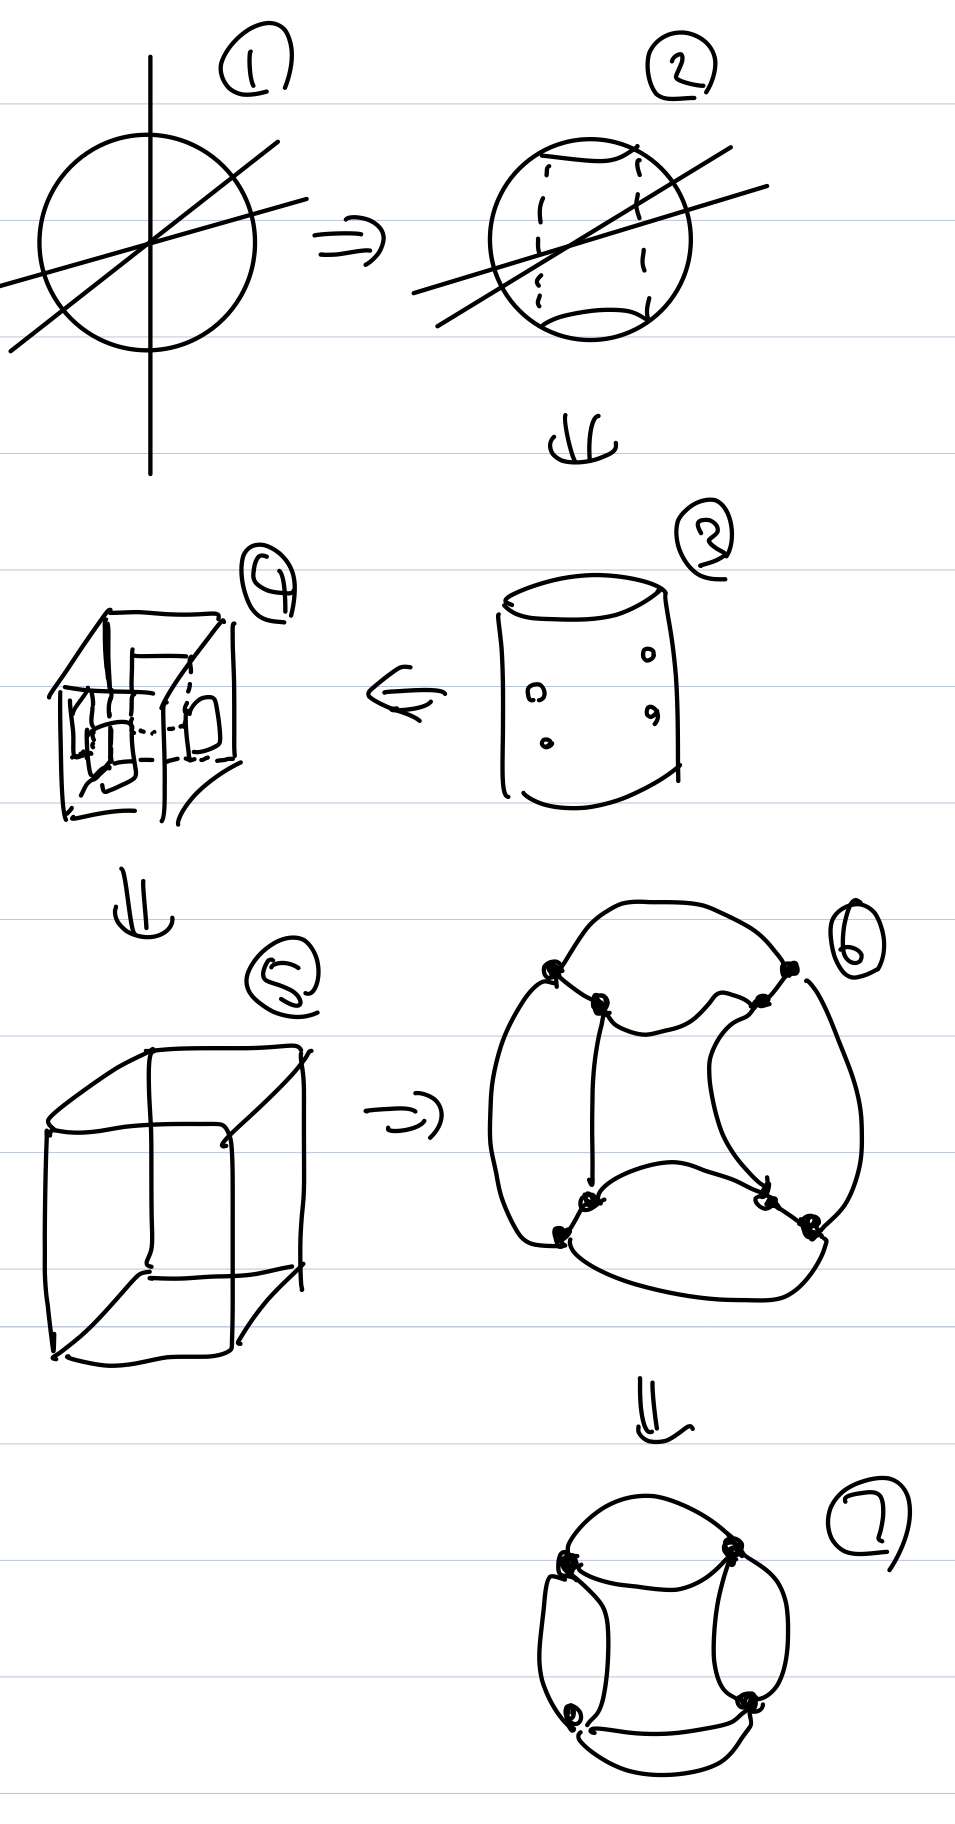
\includegraphics[width=\linewidth]{sphere_lines.jpeg}
      \caption{Problem 4, Chapter 1.2}
    \label{fig:maps}
  \end{figure}

\end{proof}

\end{document}


